\documentclass[12pt]{scrreprt}
\usepackage{graphicx}
\usepackage[font=small,labelfont=bf]{caption} 
\usepackage{titlepic}

\graphicspath{{./img/}}

% Title Page
\title{Deliverable \#1}
\author{Team D\'evlopp}
\titlepic{
\includegraphics[width=0.6\textwidth]{logo.png}}


\begin{document}
\maketitle
\tableofcontents

\section{The team}
We are team D\'evlopp. Our logo can be seen on the title page.

\subsection{Team photos}
\begin{center}
	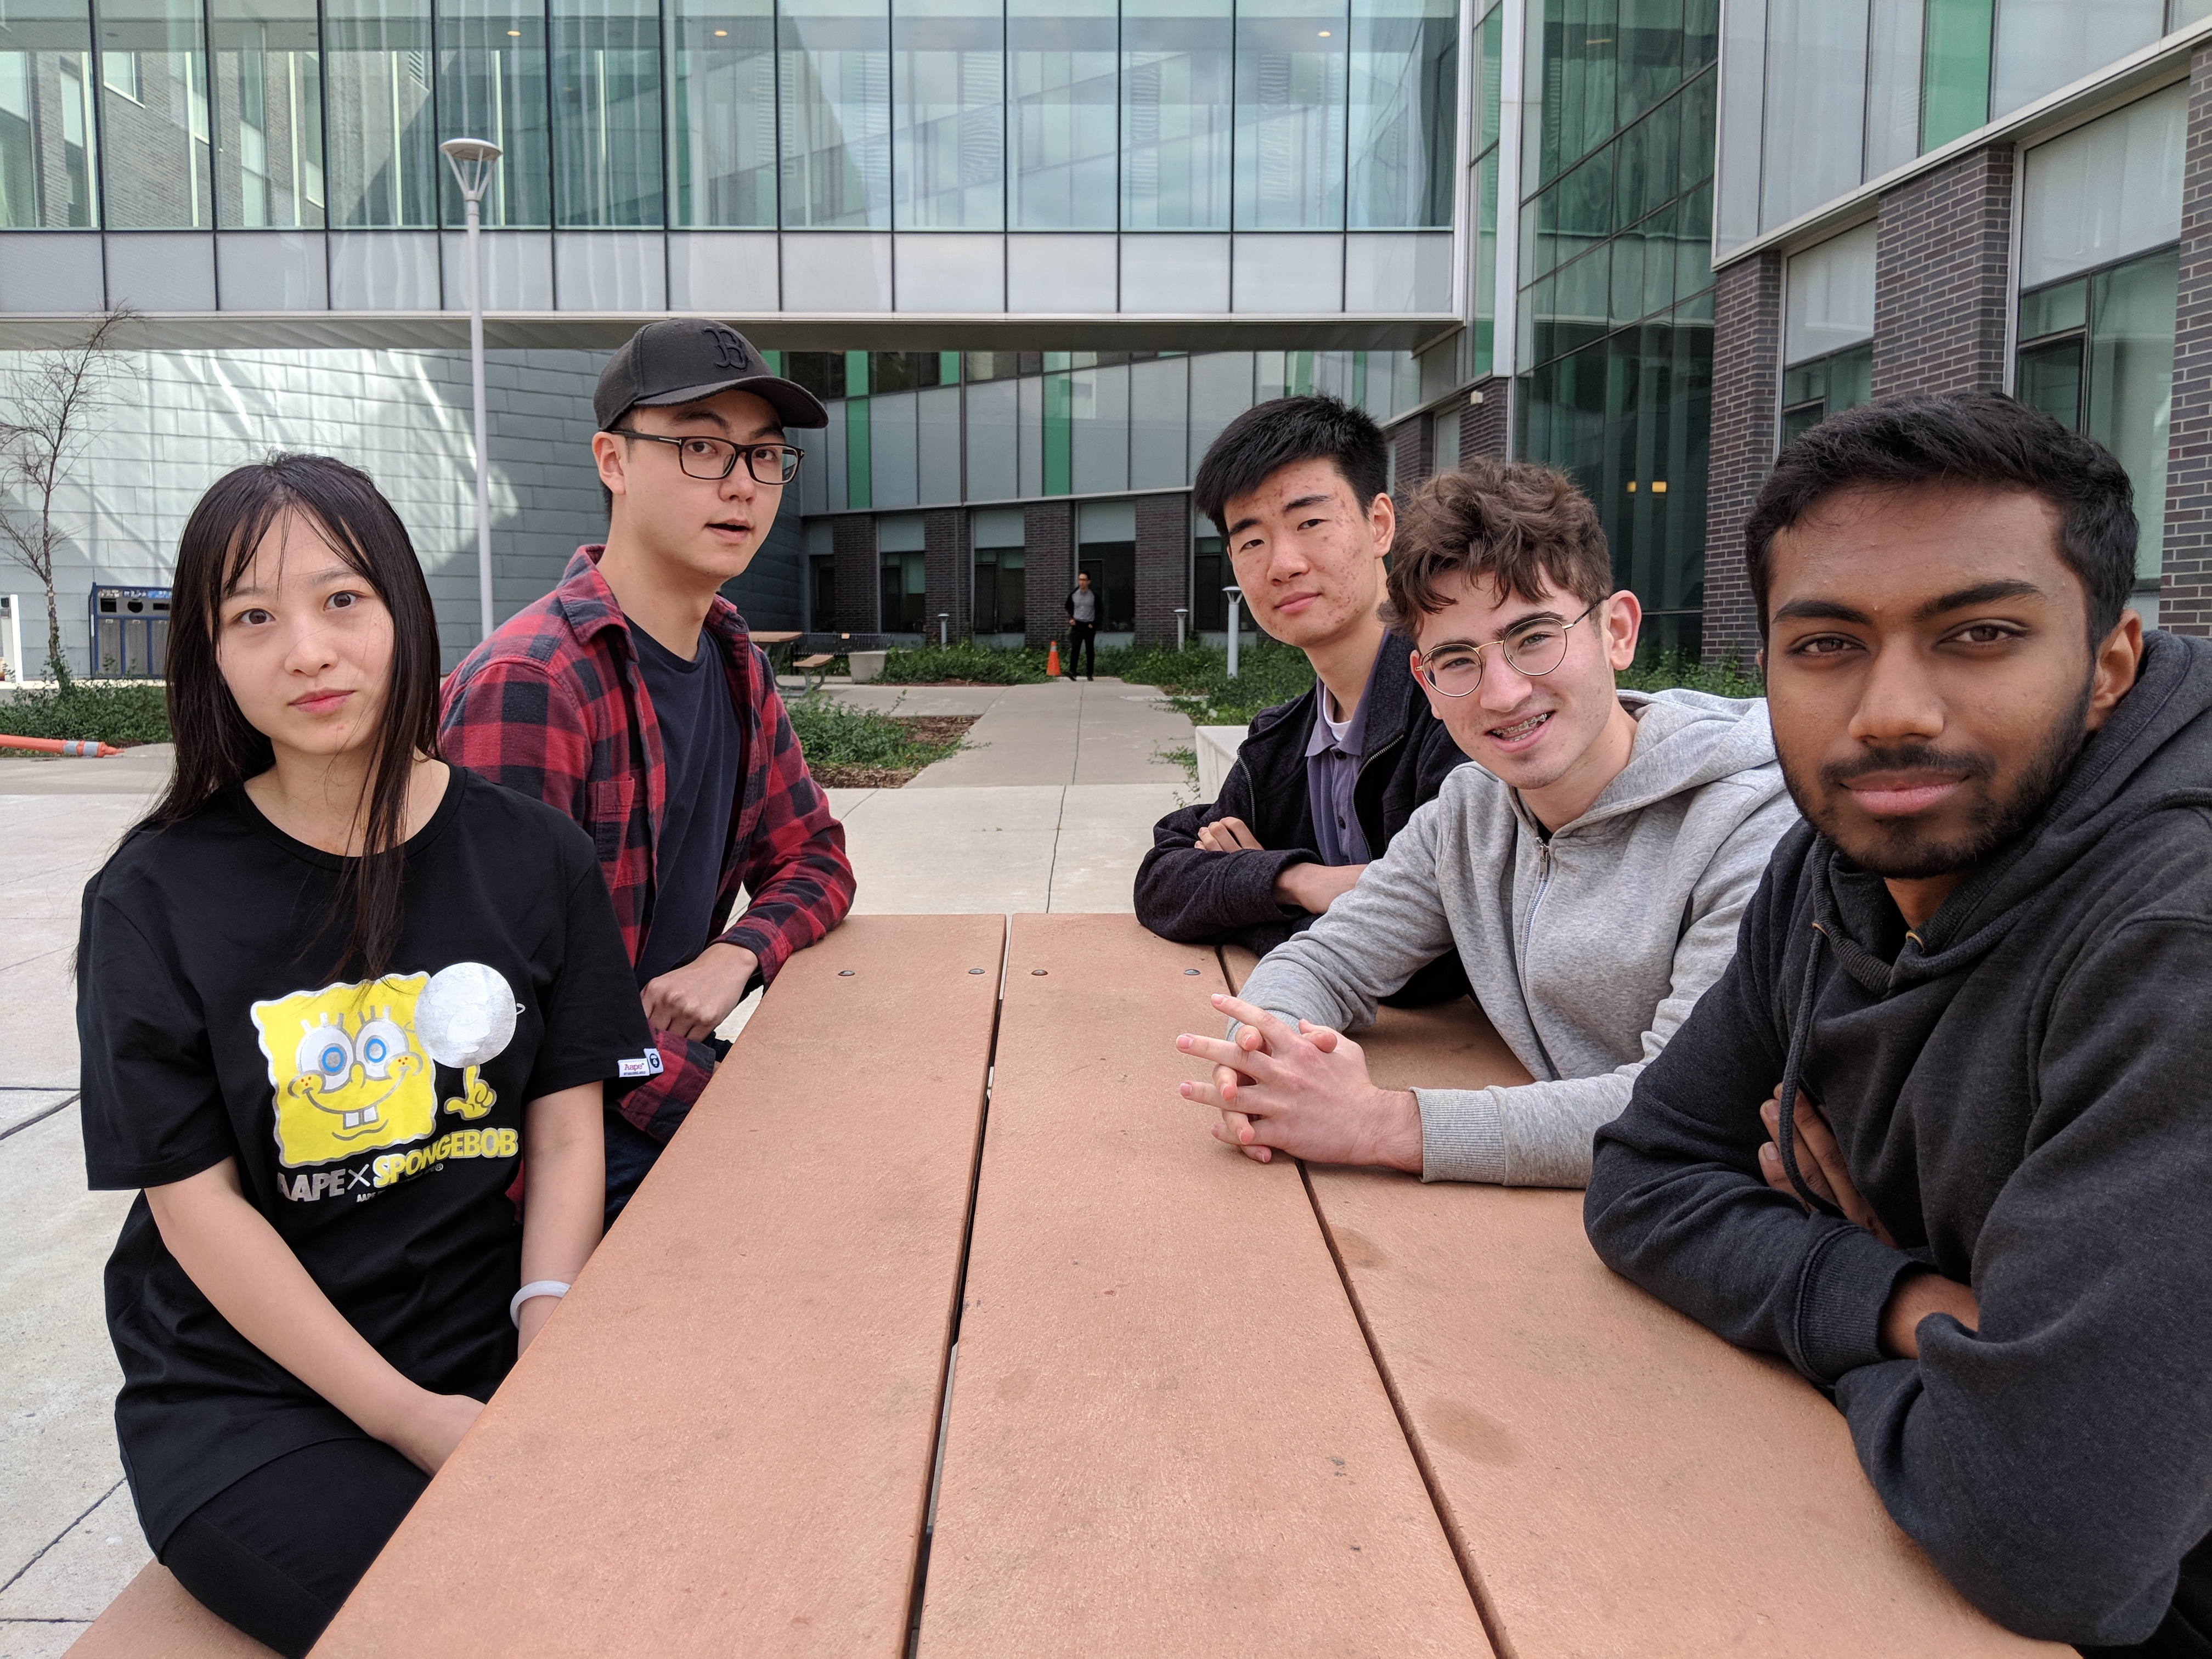
\includegraphics[width=0.9\textwidth]{team.jpg}
	\captionof{figure}{Photo of the whole team}
	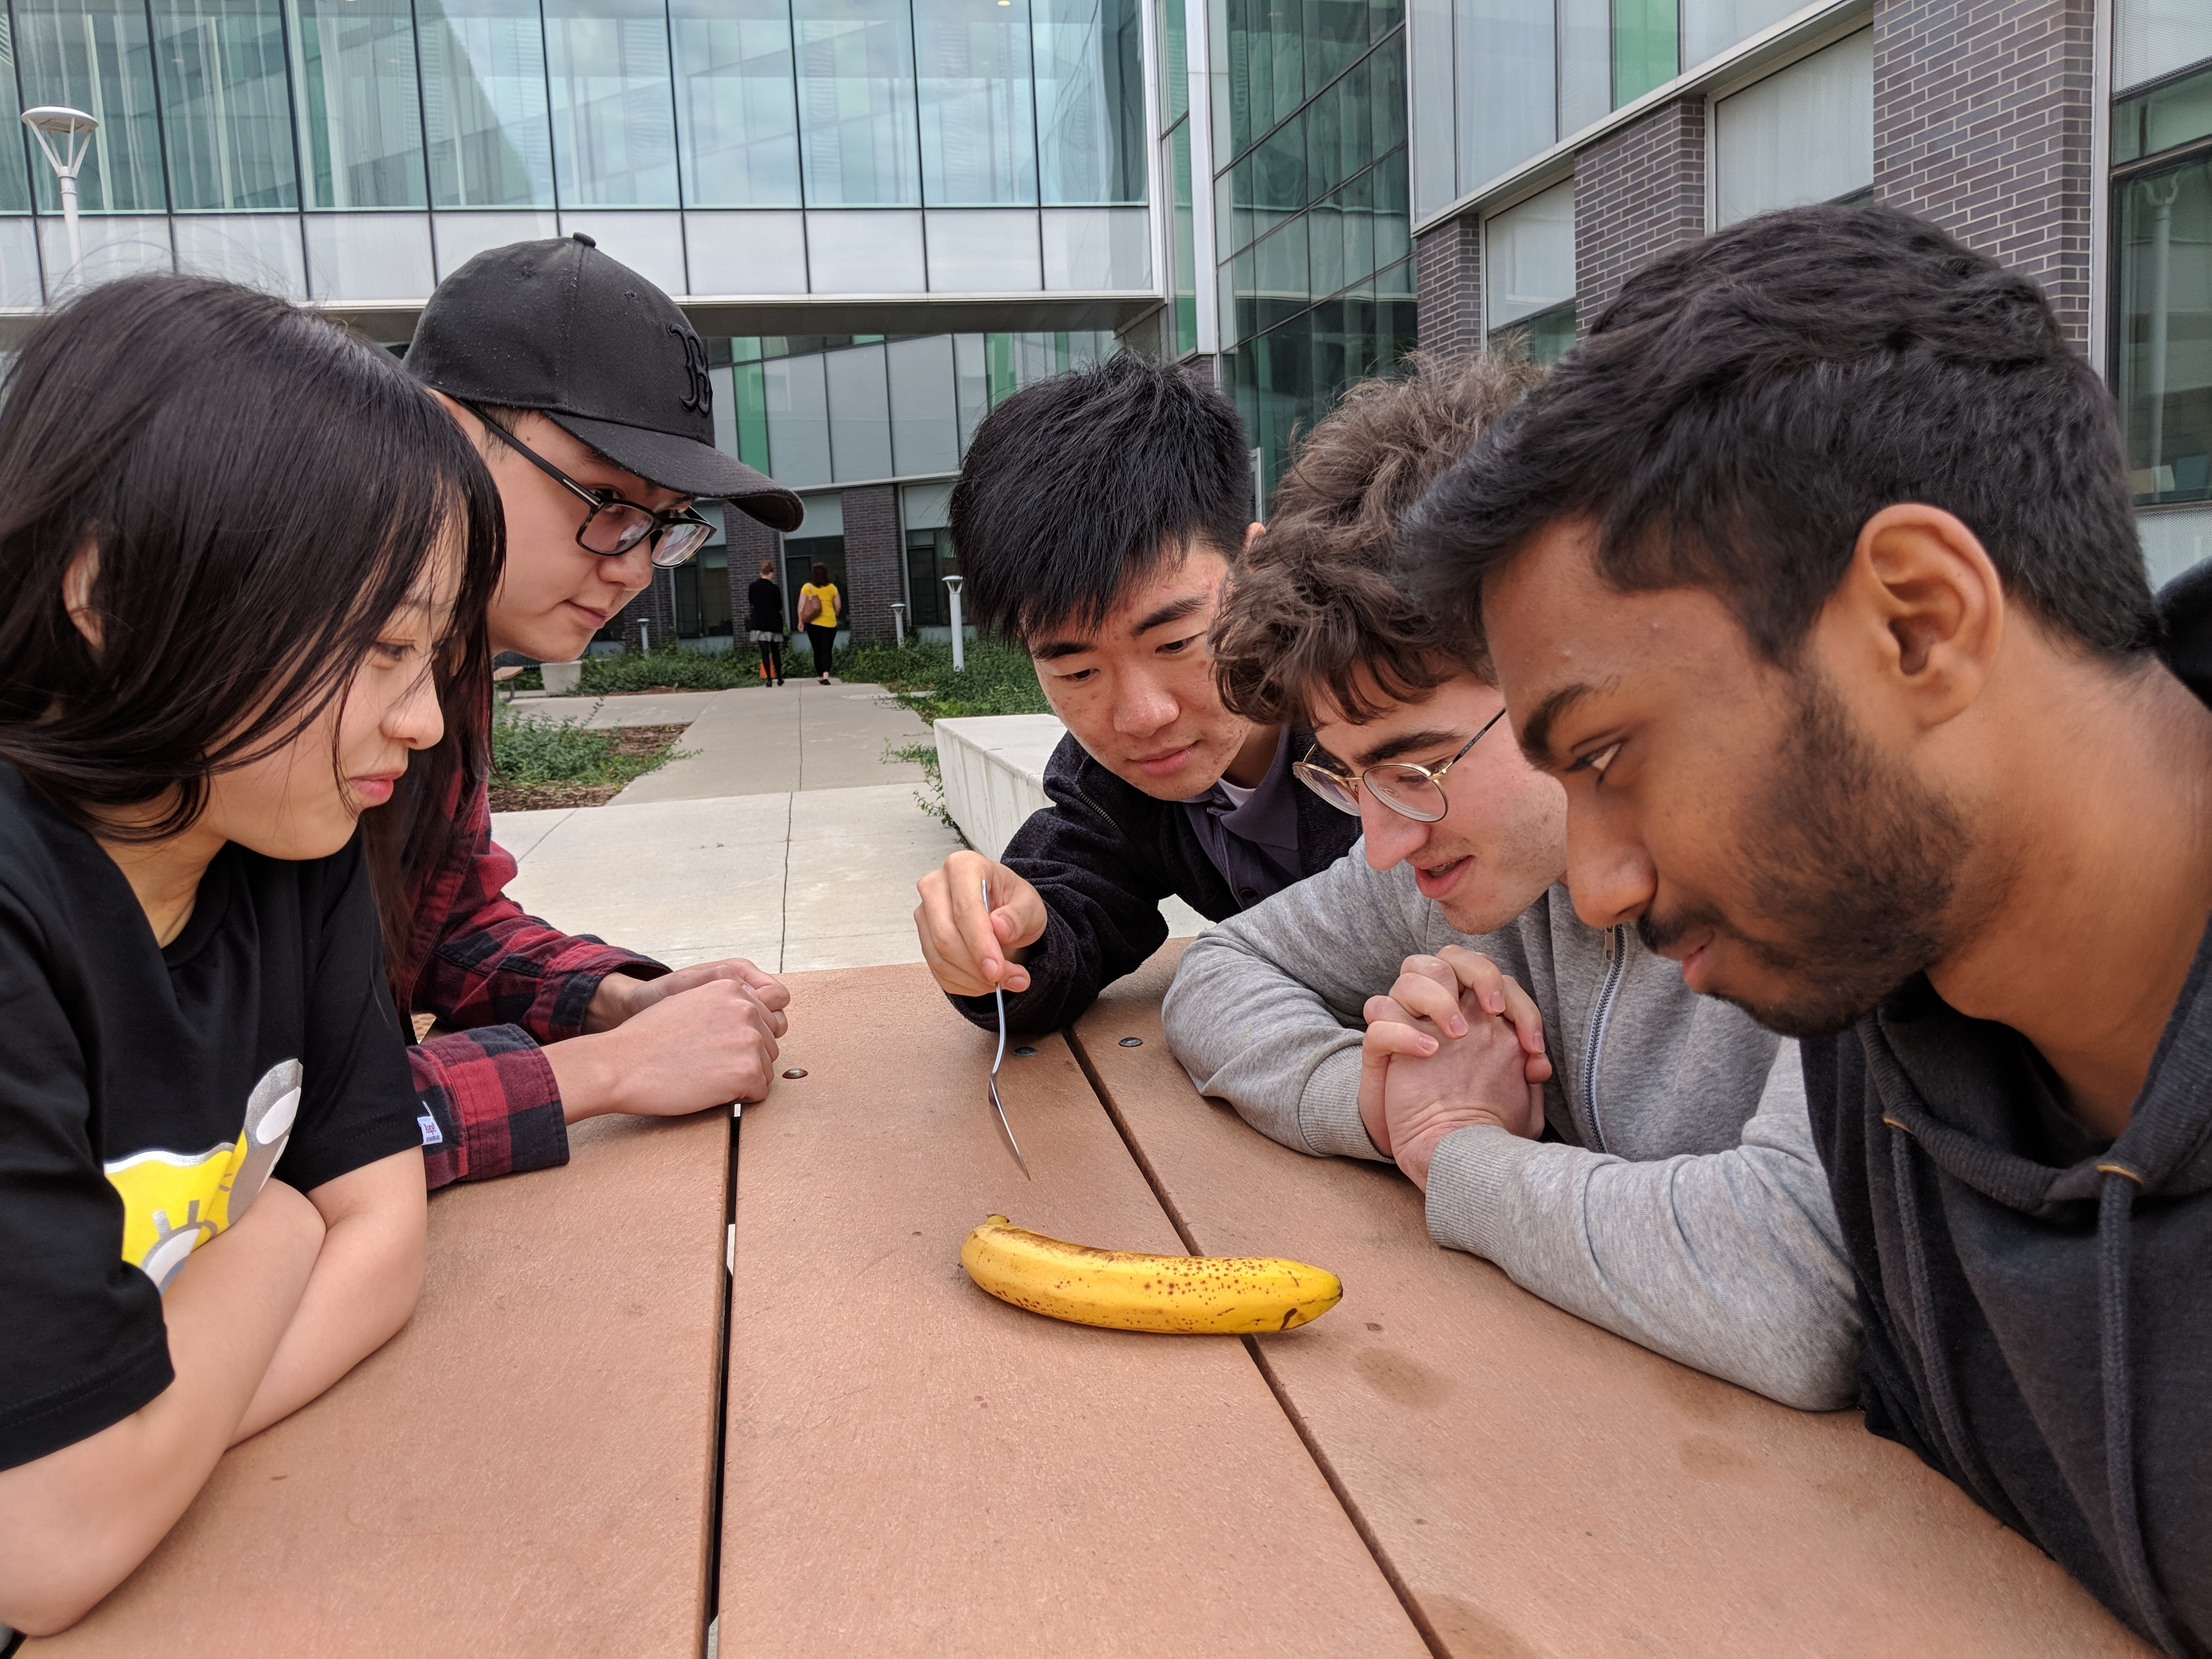
\includegraphics[width=0.8\textwidth]{food1.jpg}
	\captionof{figure}{Photo of team anticipating the consumption of a banana.}
	\vspace{0.5cm}
	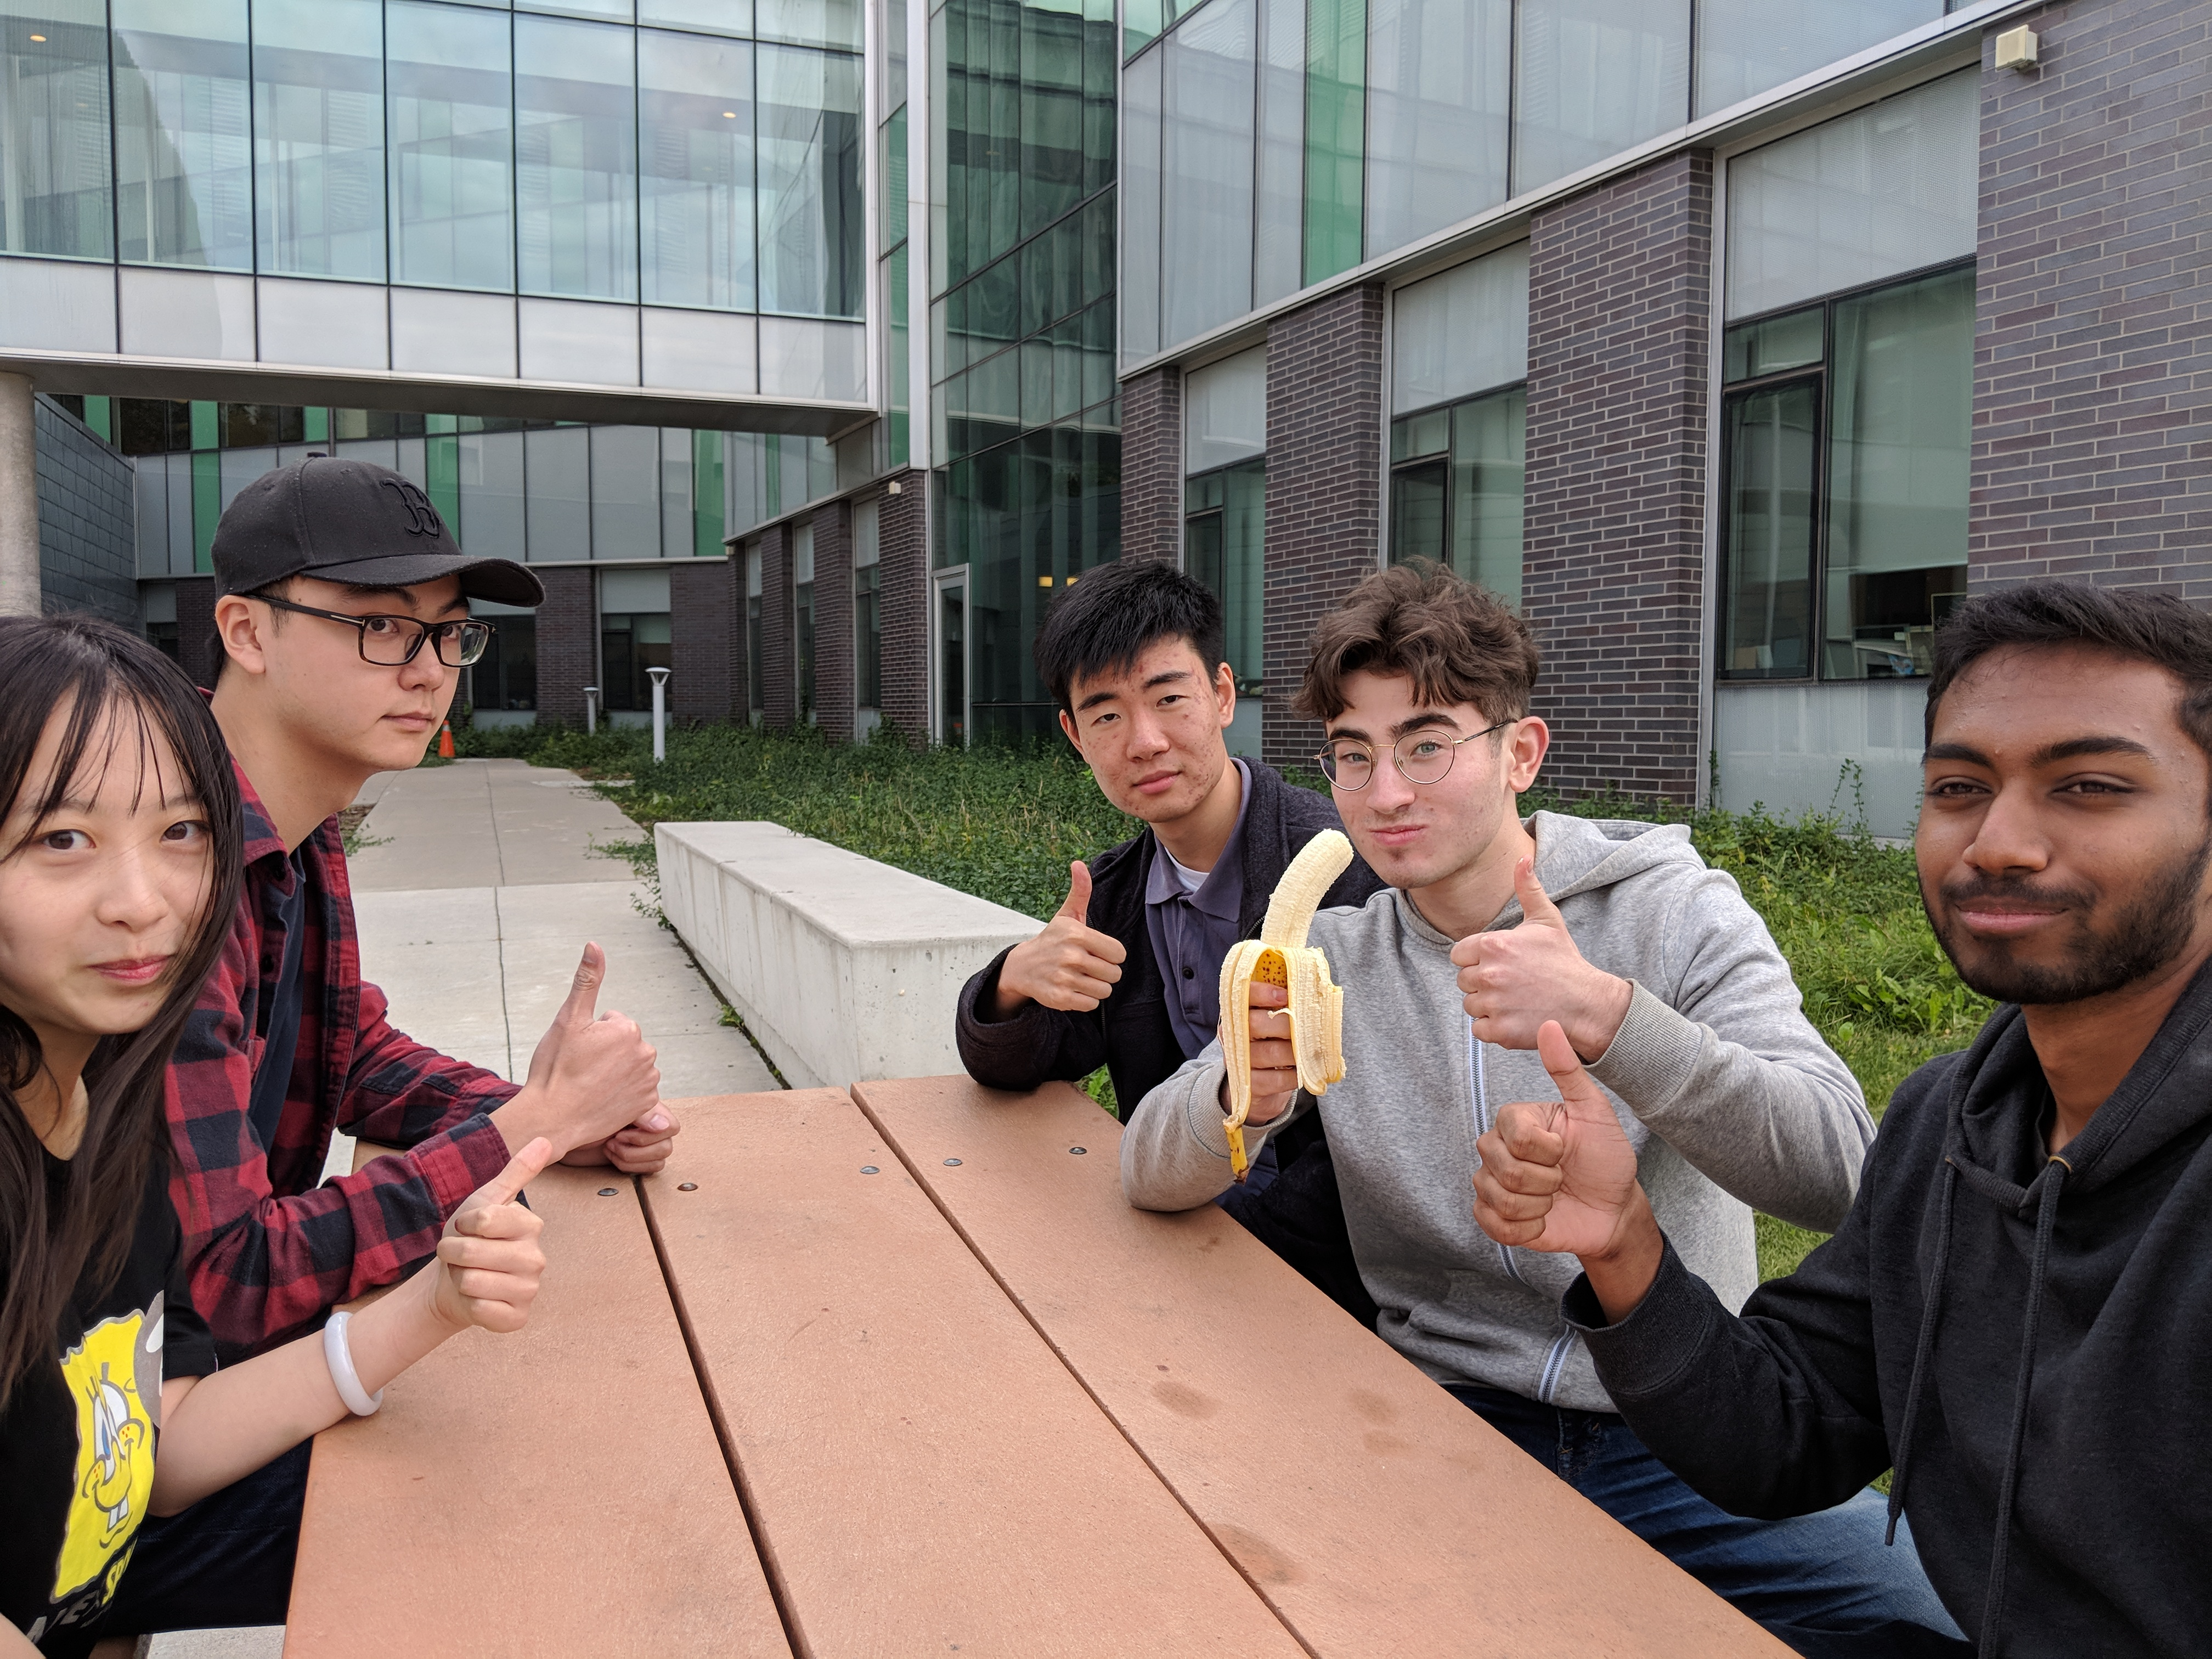
\includegraphics[width=0.8\textwidth]{food2.jpg}
	\captionof{figure}{Consumption of banana.}
\end{center}

\subsection{Our goals}
\begin{enumerate}
	\item Create a product that exceeds client expectations
	\item Use Agile practices to be an efficient, productive and organised team
	\item Improve existing skills and knowledge of software tools
	\item Learn new technologies and gain experience using them
	\item Establish rapport with client to have productive discussions of requirements
	\item Develop understanding of client needs to predict and anticipate features
\end{enumerate}

\subsection{Our strengths}
We are a diverse group of individuals, each with unique skills and experiences that help push at the boundaries of what we can achieve. Collectively, our team speaks 7 different languages: English, French, Spanish, Russian, Mandarin, Cantonese and Japanese. With each language comes a deep knowledge and understanding of the people who speak it, and their culture. This will help us create products that have much more target users, and as a result more active users.

We are good with people, but even better with technology. The whole team is fluent in Java and Python, and have experience using them in large software projects. A few of our team members know how to set-up and use databases, enabling us to add more complex features to our software. Not only have we used these skills for course work, but also in real work environments. Two of our team members, Jeffrey and Ashley have completed coop work terms. Jeffrey was a QA intern at OPS (Ontario Public Service), and Ashley completed a QA intern-ship at OTTP (Ontario Teachers' Pension Plan). Together, they bring in a year's worth of expertise in the public service field. Their experience and wisdom will be invaluable for our teams success. 

We are skilled individually, but even more as a team. All of us have had experience working in Agile teams during B07. Some of us have also had Agile experience during coop work-terms. Agile knowledge will help us squeeze out as much as possible from our team.

Finally, the team has no known food allergies. We have yet to figure out how this is relevant to our project, but we are certain that it will prove useful in the future.

\section{Meet the team}


\end{document}          
